\chapter{Orbiter}

\section{Orbital Parameters}

\section{Design}

\subsection{Instruments}

* Telescope

\subsection{Shielding}

\subsection{Thermal design}

\section{Determination of Landing Site}

\subsection{Edge detection} % KSL

* Save all images in greyscale
* Use edge detection
* Convert to binary image
* Evt. Object detection and crop image
* Laplacian Gaussian filter

\begin{figure}[htb]
	\centering
	\subfloat[TODO: Caption]{
		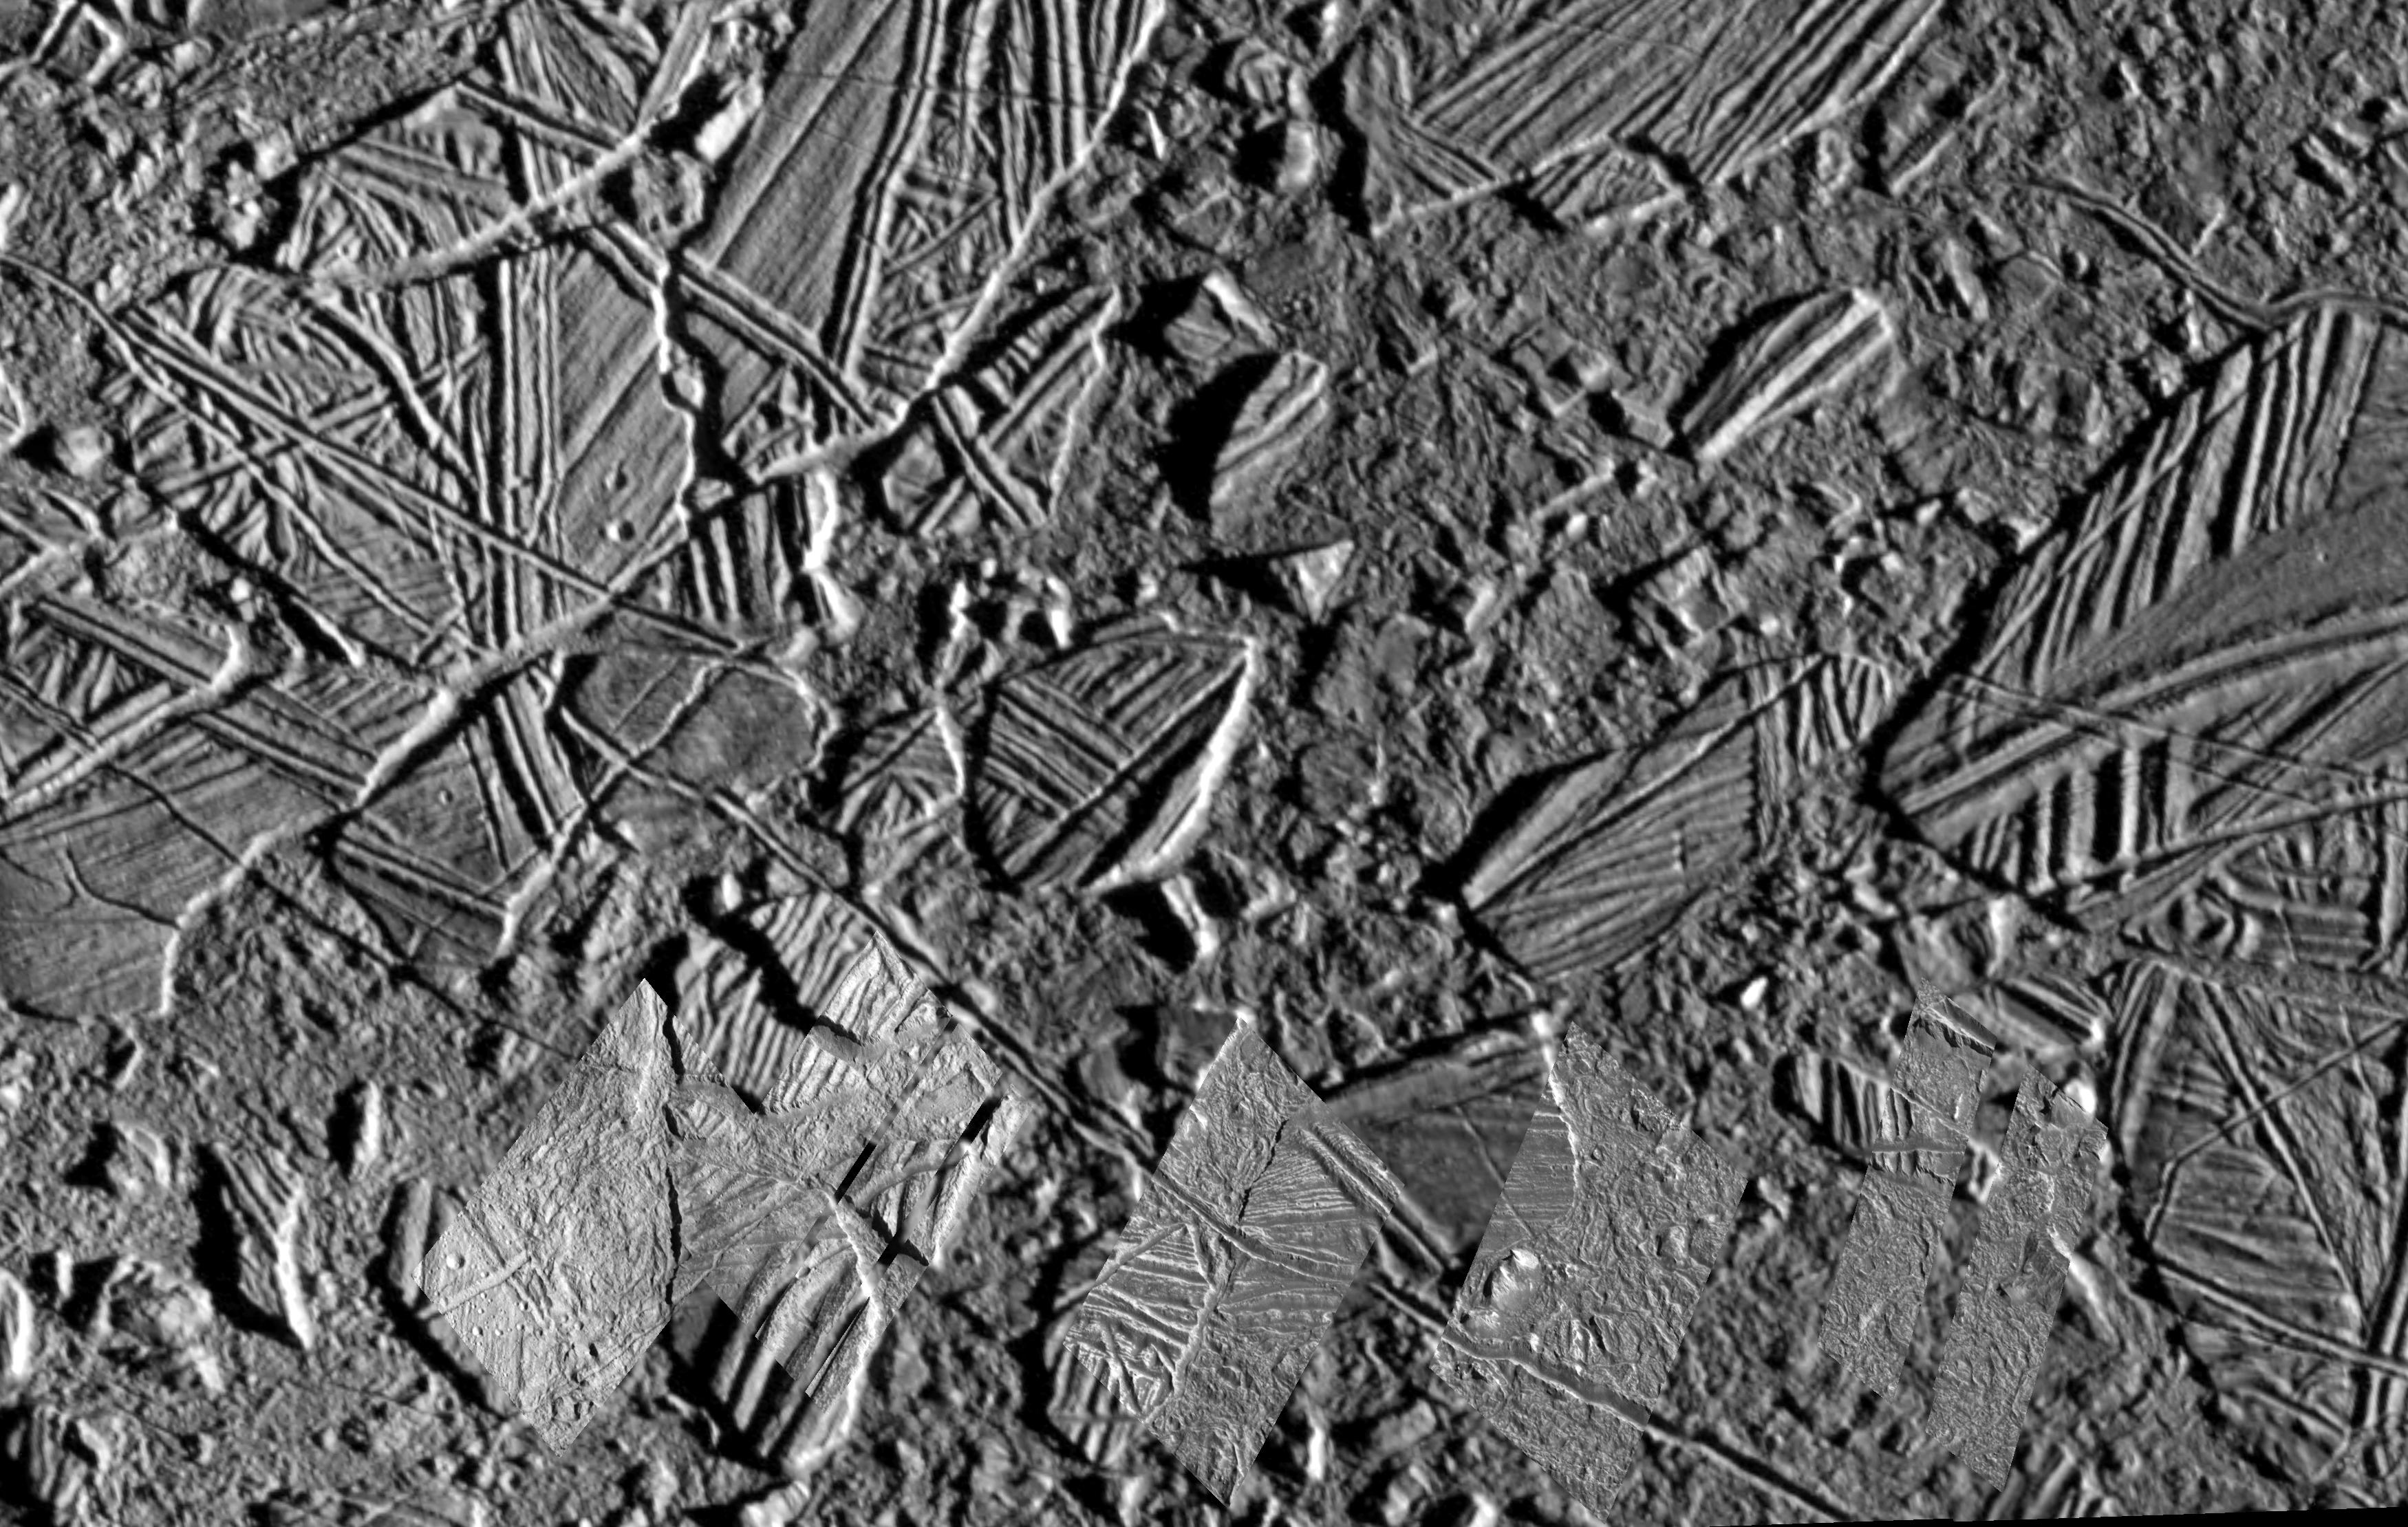
\includegraphics[width=.48\textwidth]{figures/edge/PIA01403}
	}
	\subfloat[TODO: Caption]{
		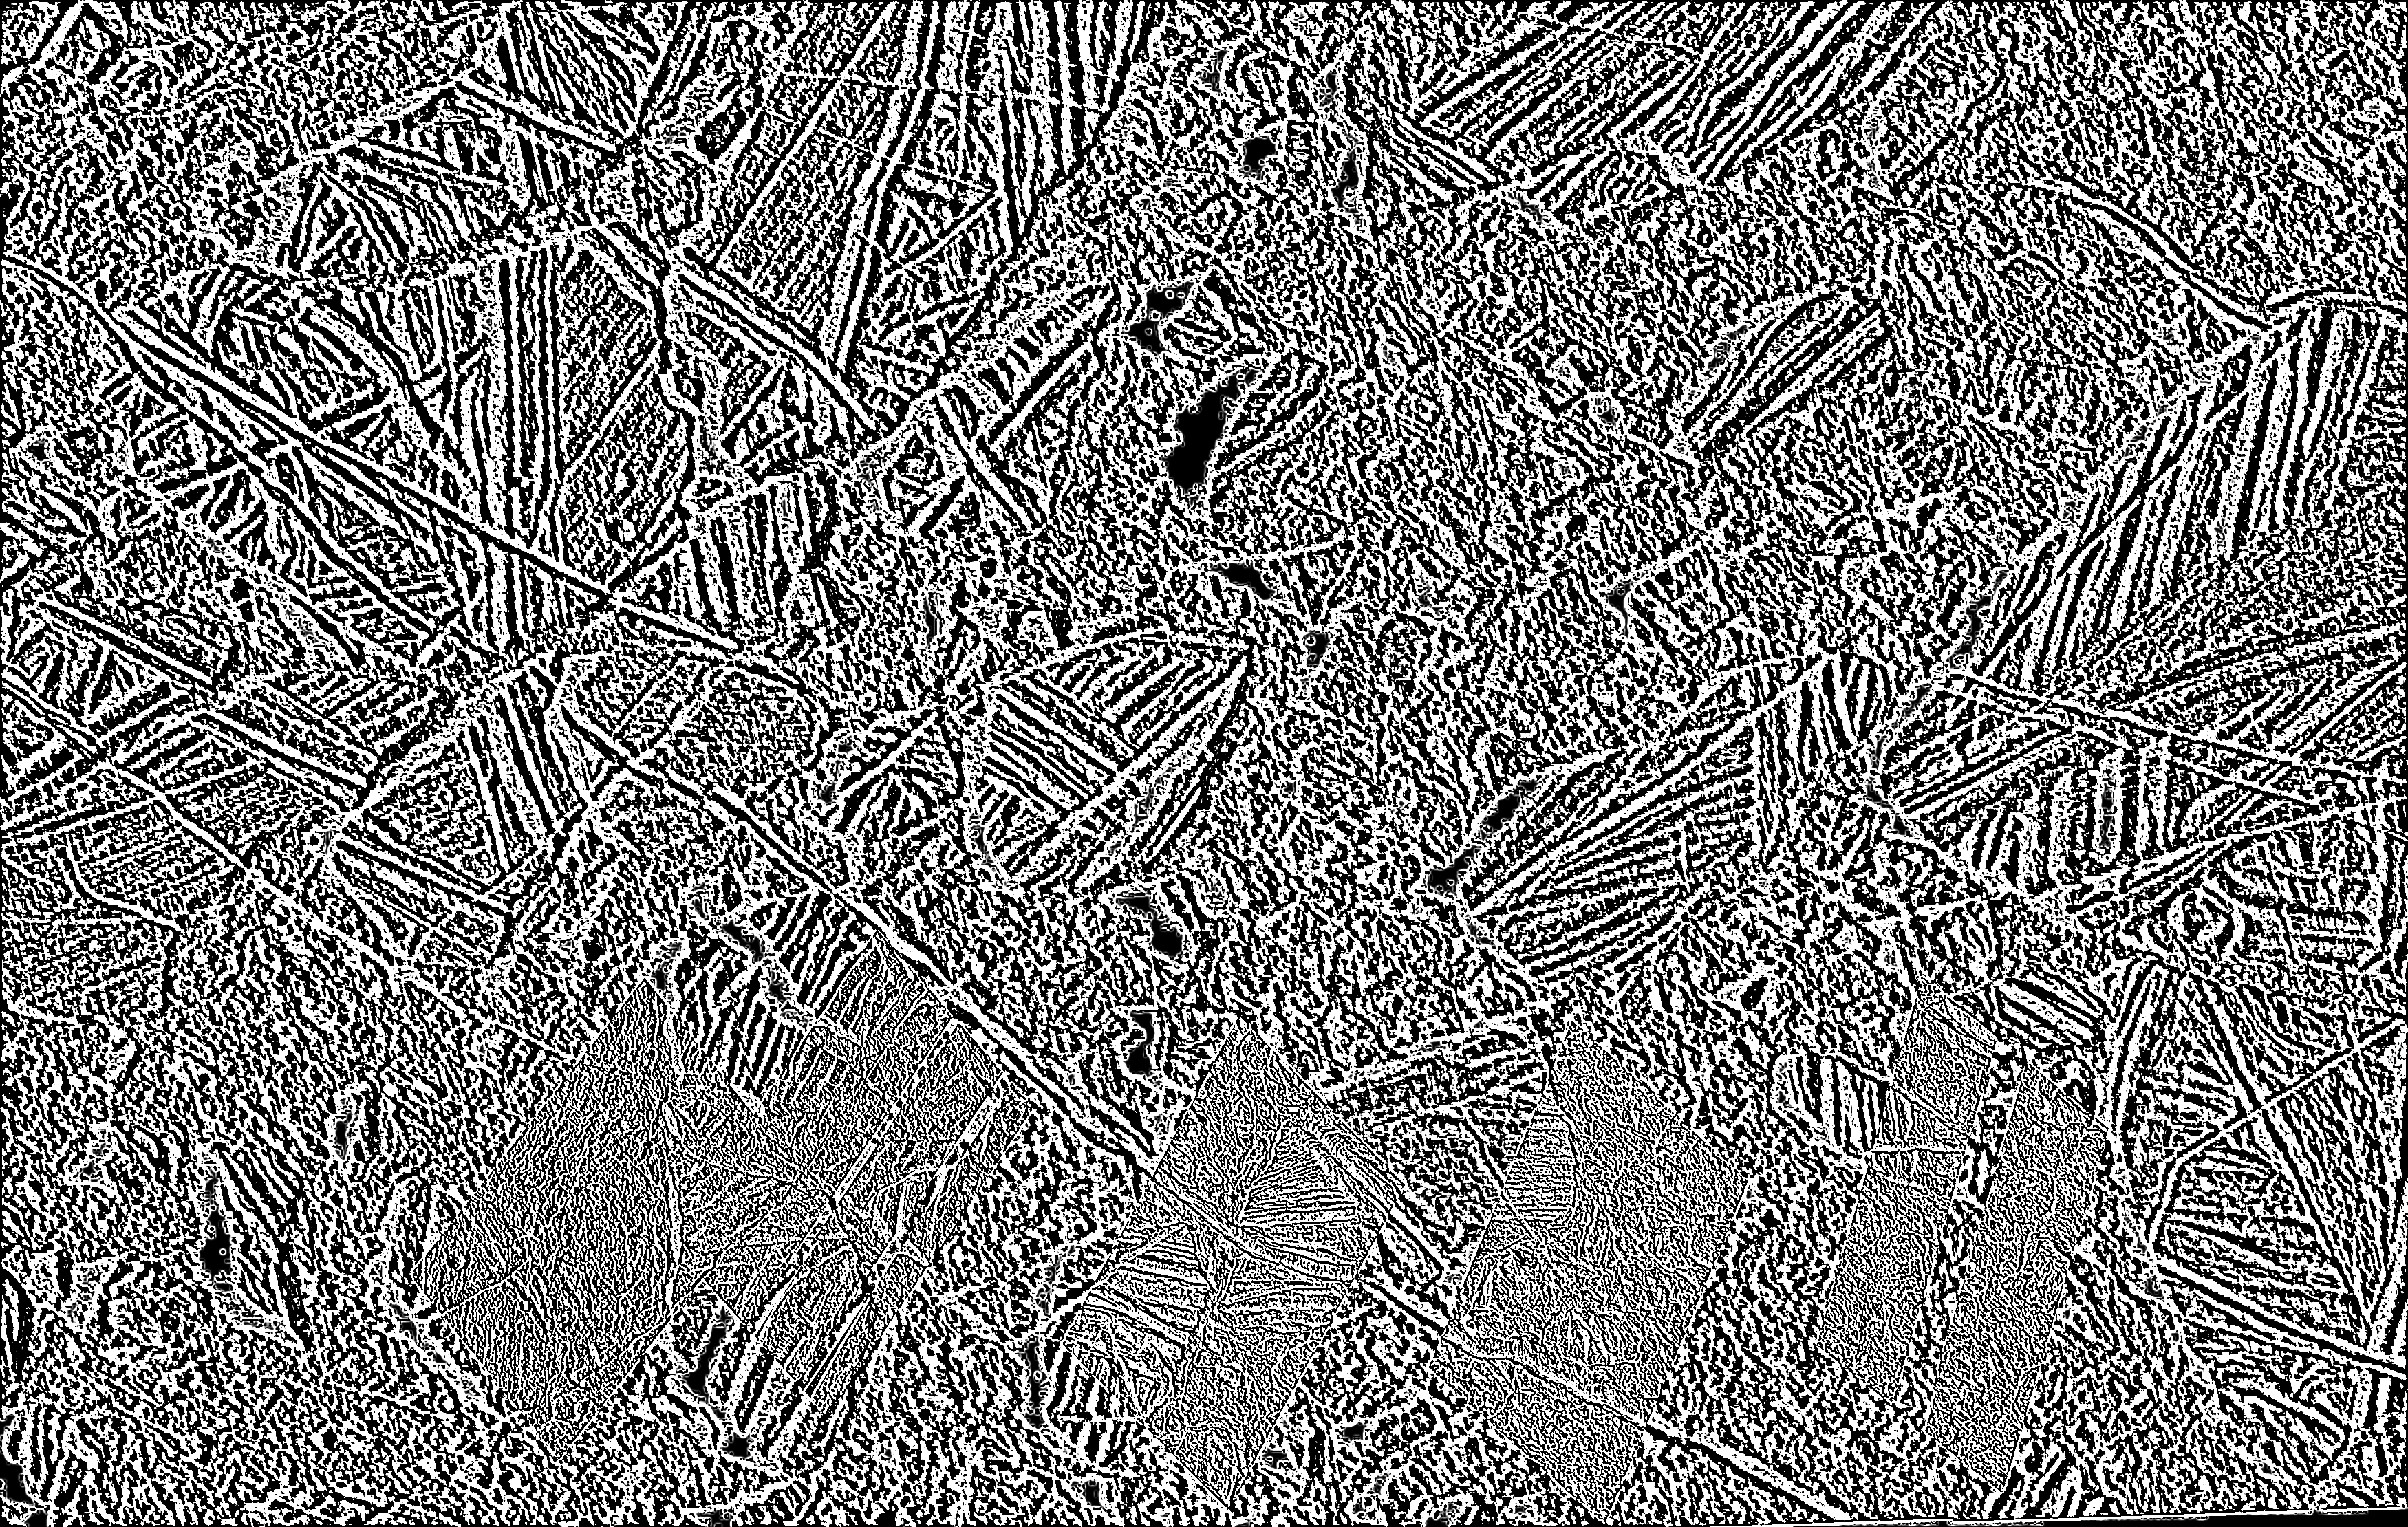
\includegraphics[width=.48\textwidth]{figures/edge/PIA01403_filtered}
	}
	\caption{TODO: Caption}
	\label{fig:PIA01403}
\end{figure}

\begin{figure}[htb]
	\centering
	\subfloat[TODO: Caption]{
		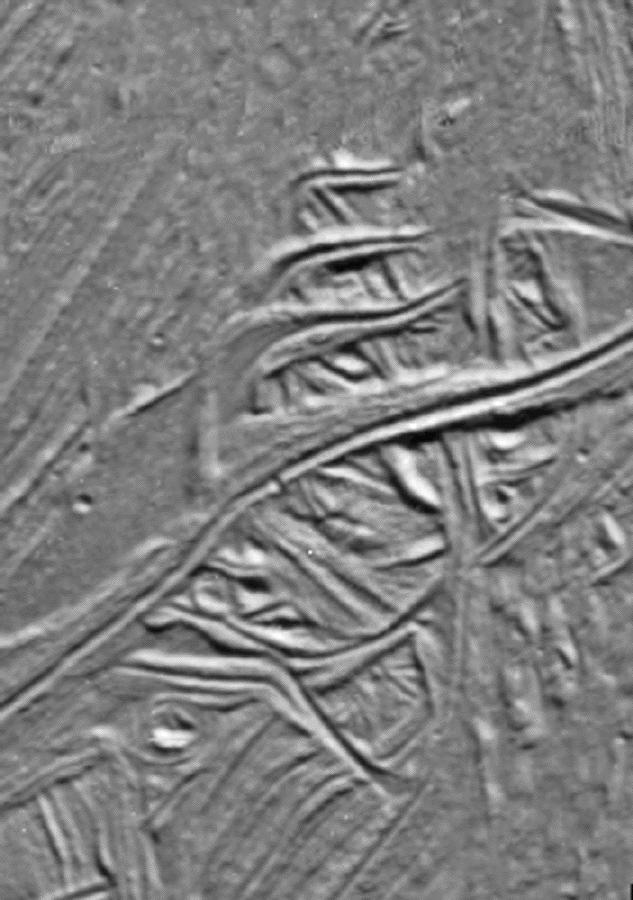
\includegraphics[width=.3\textwidth]{figures/edge/PIA01642}
	}
	\subfloat[TODO: Caption]{
		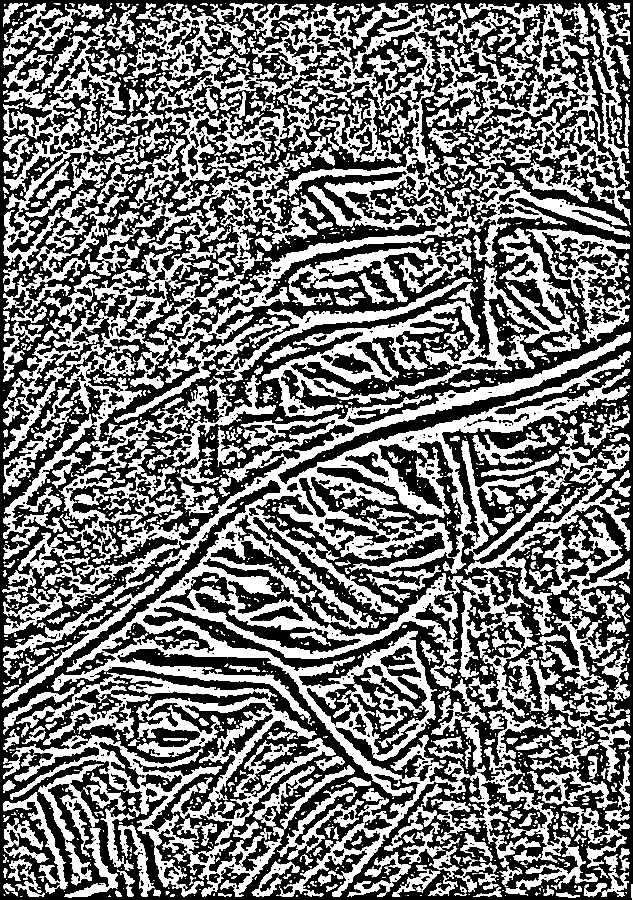
\includegraphics[width=.3\textwidth]{figures/edge/PIA01642_filtered}
	}
	\subfloat[TODO: Caption]{
		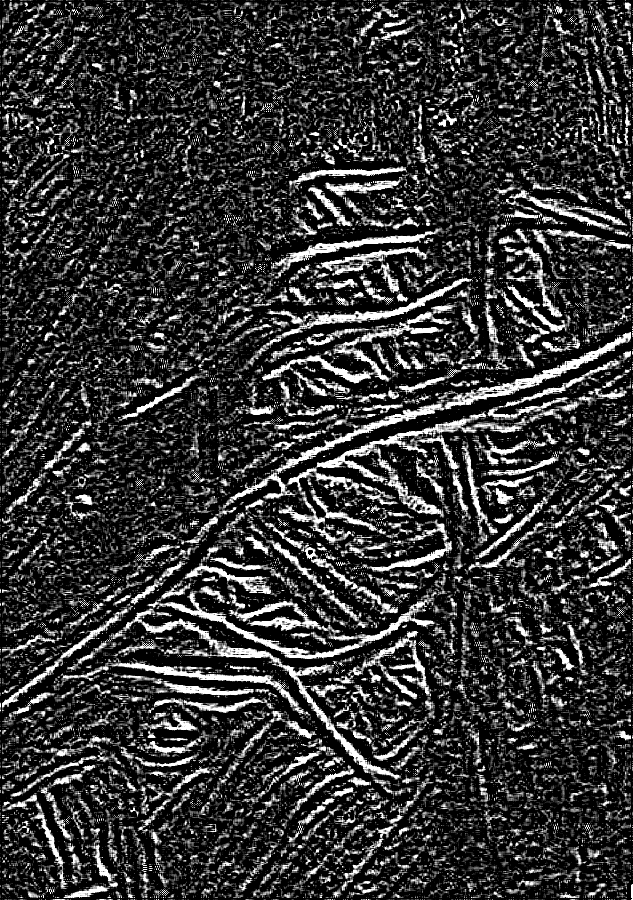
\includegraphics[width=.3\textwidth]{figures/edge/PIA01642_filtered_alternativ}
	}
	\caption{TODO: Caption}
	\label{fig:PIA01642}
\end{figure}

\subsection{Mapping of the moon}

\subsection{Europa Coordinate System}

* How to determine the ice thickness?

* Thinnest ice, smooth area, no boulders, avoid craters

* Radiation
